\part{Symmetries and Stabilizer Tensor Theory}

\section{Introduction}
In quantum theory, one predicts experiments by performing calculations involving the processes that transform the mathematical representative of a quantum system, such as operators on a state space or an observable.  This mathematical structure has proven very rich, and consequently well studied.  It is often the case that mathematical structures, such as symmetries or other algebraic properties, allow us to understand much more about a situation at hand.  

The theory of Penrose tensor networks leverages one to study the mathematical structure formed by the composition of processes themselves. Tensor networks are not just a new conceptual tool, but in fact are becoming applicable across a range of disciplines.  Primarily they have practical applications in the context of condensed matter and many-body physics.  There are still fundamental questions related to these tools, left almost entirely unexplored.  

In this lecture, we will examine some basic aspects of symmetry in tensor network states.\mn{When describing known results in quantum information, tensor network practitioners should hope to find simple and elegant rewrites between structurally intuitive and aesthetically pleasing representations.}

\section{Symmetries in Tensor Network States}

Let $\psi^{ijk}$ be a tensor with valence-(3,0).  In the graphical tensor notation of Penrose \cite{Penrose} (who also often used triangles to depict quantum states) we represent this as  
\begin{center}
 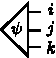
\includegraphics[width=0.07\textwidth]{psi-3}
\end{center}
When we refer to tensor symmetry, we typically mean under index exchange.  Formally, 

\begin{definition}[Exchange or index symmetric]
\label{def:ex-symmetry}
 A valence-($n$,$m$) tensor is {\it wire exchange symmetric} if one can exchange any of the arms amongst themselves, or any of the legs amongst themselves, with the effect leaving the tensor unchanged.  
\end{definition}

\begin{definition}[Full symmetry]
\label{def:full-symmetry}
A valence-($n$,$m$) tensor is {\it fully symmetric} if in addition to being exchange symmetric per Definition \ref{def:ex-symmetry}, the tensor is left invariant under arm and leg exchange. 
\end{definition}

\begin{remark}[The trivial representation]
 An exchange symmetric tensor of valence-($n$,$m$) carries the trivial representation of the symmetric group of order $n!$ (arm exchange symmetric) and order $m!$ leg exchange symmetric.  
\end{remark}

The diagrammatic generator of the symmetry group is expressed in (a).  
\begin{center}
 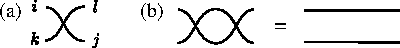
\includegraphics[width=0.5\textwidth]{symmetric-generator-I}
\end{center}
Here (a) represents the tensor $\delta^i_j\delta^k_l$ and (b) represents the contraction 
\begin{equation}
  (\delta^i_j\delta^k_l)(\delta^i_j\delta^k_l)=\delta^i_i\delta^k_k.   
\end{equation}
In diagrammatic form, this 
exchange operator is used to generate the group of operators $S_1$ in (a), $S_2$ in (b) and $S_3$ of order $3!$ in (c).  
\begin{center}
 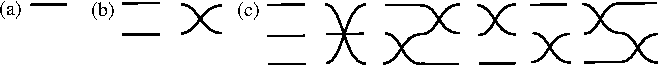
\includegraphics[width=.8\textwidth]{symmetric-group}
\end{center}

Returning now to $\psi^{ijk}$.  The state $\psi^{ijk}$ is index symmetric provided it is left invariant when acted on with any operator from (c) above.  

\begin{remark}[Symmetry breaking]
 Contraction of symmetric tensors breaks symmetry.  Given two tensors $\Gamma_1$ and $\Gamma_2$ satisfying Definition \ref{def:full-symmetry} the contraction of $\Gamma_1$ and $\Gamma_2$
 over one or more indices is not necessarily symmetric.  Examples abound.  The sum of tensors (defined for tensors of the same valence) is symmetric.
\end{remark}

\paragraph{Symmetrizers.}
Let us consider methods to perform the symmetrization of tensors.  In the definition we avoid clutter by letting the reader 
figure out how the group should act on the arms and legs of the tensor.  

\begin{definition}[Symmetrizer]
 Let us define the operator, acting on appropriate types 
 \be 
 R_G:\Gamma \mapsto \frac{1}{|G|}\sum_{g\in G} g\{\Gamma\}
 \ee 
 then $R_G\{\Gamma\}$ is necessarily symmetric under the group $G$.  
\end{definition}

\begin{example}[Example of symmetrization]
Consider $\phi^{ijk}$ which is not necessarily symmetric.  We will symmetrize the first two indices labeled 
$i$ and $j$ under $S_2$.  In this case we find 
\be 
R_G\{\phi^{ijk}\}= \frac{1}{2}\phi^{ijk} + \frac{1}{2}\phi^{jik}. 
\ee
The shorthand notation for this procedure and expansion is to write round brackets over the indices we are symmetrizing as $\phi^{(ij)k}$.  
\end{example}

\begin{remark}[Symmetrization can vanish]
 It is possible to have a tensor vanish under $R_G$.  
 Examples include the antisymmetric state $\psi_\epsilon = \ket{01}-\ket{10}$.  
 Here 
 \be
 R_G\{\psi_\epsilon^{~ij}\} = \frac{1}{2} \psi_\epsilon^{~ij} +\frac{1}{2} \psi_\epsilon^{~ji} = \frac{1}{2} \psi_\epsilon^{~ij} - \frac{1}{2} \psi_\epsilon^{~ij}. 
 \ee 
\end{remark}

\begin{example}[Symmetric over other groups]
 We have defined $R_G$ in a way where we can pick groups $G$ other than the symmetry group acting on the tensor indices.  Consider say 
 $G=\{H\otimes H\otimes H, \I\}$ where $H^2=\I$ is the standard Hadamard transformation.  We consider the valence-(1,2) \COPY-tensor $\delta^i_{~jk}$ and let $R_G$ act as 
 \be 
   R_G\{\delta^i_{~ij}\} = \frac{1}{2}\delta^i_{~jk} + \frac{1}{2}\oplus^i_{~jk} 
 \ee 
here $\oplus^i_{~jk}$ and from now on, $\oplus^i_{~jk}$ denotes the \XOR-tensor.  The resulting tensor still has three indices.  This operation is given diagrammatically as 
\begin{center}
 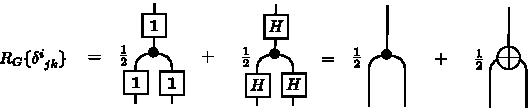
\includegraphics[width=.75\textwidth]{copy-plus-xor}
\end{center}
\end{example}

\paragraph{Antisymmetrizers.}  One can also consider antisymmetrizers. These are used regularly in the study of fermionic particles for instance.  

\begin{definition}[Antisymmetrizer]
 We define the operator of antisymmetrization as 
 \be 
 \2 A = \frac{1}{N!}\sum_{g\in S_n}(-1)^\pi g 
 \ee 
 where $\pi = 0$ for $g$ even and $\pi = 1$ for $g$ odd.  
\end{definition}

\begin{example}[Antisymmetrization]
 Consider the tensor $\Gamma^{ij}$ of valence-(2,0).  Then 
 \be 
 \2A\{\Gamma^{ij}\} =\frac{1}{2}\Gamma^{ij} - \frac{1}{2}\Gamma^{ji}
 \ee 
 and provided the tensor $\2A\{\Gamma^{ij}\}$ is non-zero, it is said to carry the sign representation of $S_2$.  It is standard to write 
 antisymmetrization over indicies, by including them in square brackets.  The example here would then be $\Gamma^{[ij]} = \2A\{\Gamma^{ij}\}$. 
\end{example}

\begin{remark}[Antisymmetrization has a non-trivial kernal]
 Examples abound of tensors which map to zero under $\2A$.  For example, there is no fully antisymmetric tensor on $(\7C^{2})^{\otimes 3}$.  
\end{remark}

\begin{example}[Considering other groups]
 We will let 
 \be 
 T^i_{~jk} = \delta^i_{~jk} - \oplus^i_{~jk}
 \ee 
 then if we consider action under
 \begin{equation}
     G=\{H\otimes H\otimes H, \I\}, 
 \end{equation}
we have that the action
 \begin{equation}
     H\otimes H\otimes H\{T^i_{~jk}\}=-T^i_{~jk}
 \end{equation}
and 
\begin{equation}
    \I\{T^i_{~jk}\} = T^i_{~jk}. 
\end{equation}
% So $G$ carries the sign representation on $T$.  
\end{example}

Let us now consider some of the symmetries present in the tensors we have defined in the first two lectures.  We will start with the \COPY-tensor.  
\begin{center}
 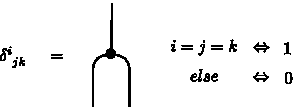
\includegraphics[width=.4\textwidth]{copy-def}
\end{center}
This is written using standard quantum theory notation as 
\be 
\sum_{ijk}\delta^i_{~jk}\ket{jk}\bra{i}. 
\ee 
As we recall, copy is fully symmetric. In addition, 
\begin{remark}[The types of possible states built from \COPY]
A concise definition of the \COPY-tensor is given as any combination of raised or lowered indices on 
 $\delta^{ijk}$, a Kronecker delta function on three indices.   
 In step, one might write the n-party \GHZ-state as 
 \be 
 \psi_\GHZ = \sum \delta^{ijk...l}\ket{ijk...l}. 
 \ee 
Tensor products of states of this form are precisely the only types of states constructible with the \COPY-tensor alone.  
\end{remark}
\begin{figure}[h]
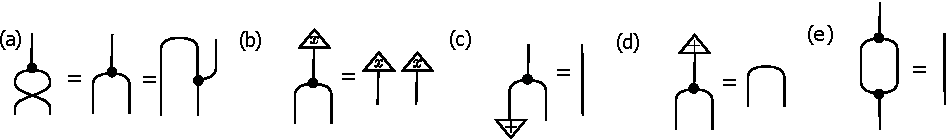
\includegraphics[width=15\xxxscale]{copy-properties1}
%\epsfig{figure=copy-properties,width=15cm}
\caption{Diagrammatic properties of the \COPY-tensor \cite{boolean03}. (a) Full-symmetry.
(b) Copy points, e.g.\ $\ket{x}\mapsto\ket{xx}$ for $x=0,1$ for qubits.  (c) The unit 
given as $\bra{+}\bydef\bra{0}+\bra{1}$.  (d) Applying the unit to the top leg creates a cap.  (e) Copy then delete is the same as identity.}\label{fig:copygate1}
\end{figure}

We are going to study these diagrammatic equations from Figure \ref{fig:copygate1} under local unitary change of basis.  
We will first define the rotation operator 
\begin{definition}[Tensor rotation operator]
 Let us define a rotation operator which acts on a valence-(n,m) tensor as follows.  On the n input arms, $U$ is applied, 
 on the m output legs, $U^\dagger$ is applied.  We will define this map as $U_G$ which is given diagrammatically as follows 
\begin{center}
 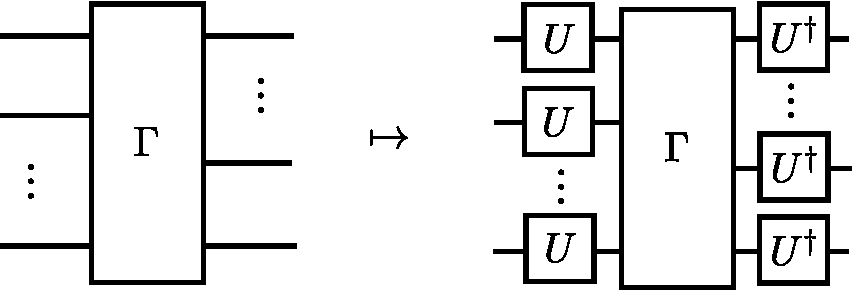
\includegraphics[width=.4\textwidth]{tensor-rotation}
\end{center}
\end{definition}

\paragraph{Rotations of \COPY-tensors.}\label{sec:generalcopy}
It is of course desirable to extend the definitions of the valence-(1,2) \COPY-tensors to act on arbitrary bases.  We would then change to a basis 
$B$ as 
 \begin{center}
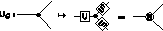
\includegraphics[width=0.60\textwidth]{lessgeneralcopy}
\end{center}


\begin{example}[Engineering a map to copy a particular basis]
Say you have an orthonormal basis $\{\ket{\psi},\ket{\psi^\bot}\}$, which we will call $\sf B$ and you wish to define a \COPY-tensor on this basis as $\ket{\psi}\mapsto \ket{\psi,\psi}$ and $\ket{\psi^\bot}\mapsto \ket{\psi^\bot,\psi^\bot}$.  To represent such a tensor diagrammatically we draw 
 \begin{center}
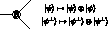
\includegraphics[width=0.40\textwidth]{generalcopy1}
\end{center}
To transform the \COPY-tensor to copy this new basis, define the unitary 
\be
U = \sum_i\ket{i}\bra{\phi_i}
\ee
where $\{\phi_i\}_i$ and $\{i\}_i$ are bases for the same space such that $\braket{\phi_i}{\phi_j}=\delta_{ij}$ and $\braket{i}{j}=\delta_{ij}$.  The map $U$ is unitary as 
\be
U^\dagger U = (\sum_i\ket{\phi_i}\bra{i})(\sum_j\ket{j}\bra{\phi_j})=\sum_j\ket{\phi_i}\delta_{ij}\bra{\phi_j}=\I. 
\ee
\end{example}

\begin{remark}
There are important cases were we only consider transforming \COPY-tensors using self adjoint unitary maps.  Hadamard is an example with
\begin{equation}
    H=\frac{1}{\sqrt{2}}(X+Z)=H^\dagger. 
\end{equation}
Every projector gives rise to such a map as $U= \I -2P$ is unitary when $P^2=P$.  The map is invertible, and hence every self adjoint unitary gives rise to a projector, illustrating the 
bijection between self adjoint unitary maps and projects.  
\end{remark}

\begin{example}[Transforming \COPY-tensors into \XOR-tensors]
 It is well known in the theory of algebra that Hadamard transforms (the Fourier transform over $\7Z_2$) relate \COPY-tensors and \XOR-tensors.  This is also known in quantum circuits.  For the higher dimensional case see \cite{BB11}.  
 The transformation of a \COPY-tensor into an \XOR-tensor is given diagrammatically as follows.  
  \begin{center}
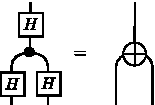
\includegraphics[width=0.20\textwidth]{copy-2-xor1}
\end{center}
\end{example}

\begin{remark}[Arbitrary rotations]
 We will now mention exactly how the general form of the diagrammatic laws can transform properly under rotation.  
The general form is straightforward.  States rotate under $U^\dagger$ and tensors rotate as we have already defined.  
\begin{center}
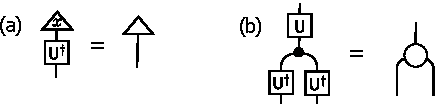
\includegraphics[width=0.60\textwidth]{rotated-copy-properties1}
\end{center}
\end{remark}

\begin{myexercise}[General rotation] 
 Prove that if the \COPY-tensor is rotated as by $U$ above, then the diagrammatic identities hold.  
\end{myexercise}

\section{The Interaction of Networks Comprised of \texorpdfstring{$\delta^{ijk}$}{} and \texorpdfstring{$\oplus^{ijk}$}{}}

We will now consider networks comprised of \COPY-tensors and \XOR-tensors.  Let us first recalls DeMorgan's law.  

\begin{definition}[DeMorgan's Law]
DeMorgan's law is a relationship between logical \AND, ($\wedge$) and logical \OR, ($\vee$).  The relationship 
is found by considering what in quantum circuit theory would be called bit flips ($X$), 
induced by logical negation ($\neg$).  The equation reads 
\be 
\neg (a \wedge b) = (\neg a)\vee (\neg b) 
\ee 
In diagrammatic form, this equation becomes 
\begin{center}
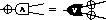
\includegraphics[width=0.45\textwidth]{demorgan}
\end{center}
we note that $X^2 = \I$. 
\end{definition}

\begin{remark}[Relating \COPY{} and \XOR-tensors]
A similar structure to the DeMorgan's law relating \AND{} and \OR-tensors also holds 
between \COPY- and \XOR-tensors.  In this case, instead of using negation, we use the Hadamard gate $H$.  
In diagrammatic form, this becomes 
\begin{center}
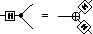
\includegraphics[width=0.40\textwidth]{copy-xor-demorgans}
\end{center}
and we note that $H^2=\I$.  
\end{remark}

To continue, let us recall the definitions of the tensor at hand.  In constraint equation form, together with graphical representations, these read as 
\begin{center}
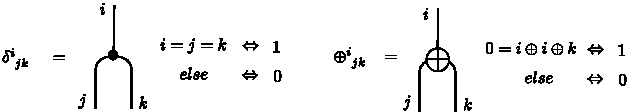
\includegraphics[width=0.910\textwidth]{copy-xor-def}
\end{center}
from the constraint equations, we can readily construct, a sort of ``truth table'', which gives the value of the tensor contraction, provided we contract the wires (labeled $i$, $j$ and $k$) with states $\ket{0}$ or $\ket{1}$.  We illustrated these possibilities in the contraction table below.  

\begin{center}
\begin{tabular}{ccc||c||c}
i         & j         & k         & $\oplus_{ijk}$ & $\delta_{ijk}$\\\hline
$\ket{0}$ & $\ket{0}$ & $\ket{0}$ & 1 & 1\\
$\ket{0}$ & $\ket{0}$ & $\ket{1}$ & 0 & 0\\
$\ket{0}$ & $\ket{1}$ & $\ket{0}$ & 0 & 0\\
$\ket{0}$ & $\ket{1}$ & $\ket{1}$ & 1 & 0\\
$\ket{1}$ & $\ket{0}$ & $\ket{0}$ & 0 & 0\\
$\ket{1}$ & $\ket{0}$ & $\ket{1}$ & 1 & 0\\
$\ket{1}$ & $\ket{1}$ & $\ket{0}$ & 1 & 0\\
$\ket{1}$ & $\ket{1}$ & $\ket{1}$ & 0 & 1
\end{tabular}
\end{center}

\begin{myexercise}[Linearity of tensor contraction]
 Tensor contraction is linear. Given the table above, use linearity to determine the contraction found from other states, such as say $\ket{+}$, $\ket{-}$, etc. 
\end{myexercise}


To consider further properties relating the interaction of \COPY-tensors and \XOR-tensors we will recall Lafont's presentation of the Boolean calculus \cite{boolean03, CTNS}, given in Figure \ref{fig:F2-presentation1}.  


\begin{myfullpage}
\begin{illexample}
\label{fig:F2-presentation1}
\begin{center}
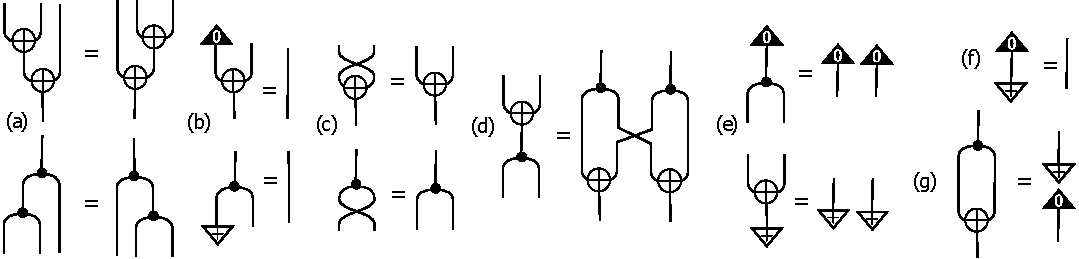
\includegraphics[width=20\xxxscale]{F2-presentation1}
%\epsfig{figure=F2-presentation,width=16cm}
%\caption{
\end{center}
Lafont's presentation of the linear fragment of the Boolean calculus \cite{boolean03}.  
(a) associativity; (b) unit laws; (c) input symmetry (as mentioned, these tensors are in fact fully symmetric 
by Definition \ref{def:full-symmetry}); (d) bialgebra law; (e) illustrates that the unit for \XOR{} is a copy point for the \COPY-tensor and vice versa; (f) the inner product $\braket{0}{+}\in\7C$.  Global scale factors are represented as blank space on the page; (g) is the Hopf law.
\end{illexample}
\end{myfullpage}

These rules, and also the algebraic properties of \XOR-algebra result in the following class of functions (the only type possible to construct using the operations at hand.  

\begin{definition}[Linear and affine boolean functions]
Linear Boolean functions take the general form
\be
f(x_1,x_2,...,x_n)=c_1x_1\oplus c_2x_2\oplus ...\oplus c_nx_n
\ee 
where the vector $(c_1,c_2,...,c_n)$ uniquely determines the function.  The affine
Boolean functions take the same general form as linear functions.  However, for functions
in the affine class, variables can appear in both complemented
and uncomplemented form. Affine Boolean functions take the general form
\begin{equation}\label{eqn:affine}
f(x_1,x_2,...,x_n)=c_0\oplus c_1x_1\oplus c_2x_2\oplus ...\oplus c_nx_n
\end{equation}
where $c_0=1$ gives functions outside the linear class.  From the identities,
$1\oplus 1=0$ and $0\oplus x=x$ we require the introduction of only one constant
($c_0$). 
\end{definition}


When contracted, \XOR- and {\sf COPY}-tensors compose to create tensor networks representing the class of linear
quantum networks. This gives rise to the following class of quantum states.  

\begin{definition}[The class of linear quantum states]
 We define the linear class of quantum states as quantum states of the form 
 \be 
 \psi_{\oplus L} = \sum c_1x_1\oplus c_2x_2\oplus ...\oplus c_nx_n \ket{x_1, x_2, ..., x_n}
 \ee
\end{definition}


\begin{myexercise}
  Here we will consider a 1D system.  What is the maximum possible $\chi$ (as defined in lecture I) in a bi-partition of a linear quantum state?   
\end{myexercise}



\begin{myexercise}[Correlations in polarity states (Optional)]
Here let us consider a state defined as 
\be 
\psi:=\sum (-1)^{f(\textbf x)}\ket{\textbf x}
\ee 
where the sum is over all $\textbf x$.  These states are often considered in quantum algorithm theory.  
Prove that $\psi$ is separable iff the function implements a linear function.  
\end{myexercise}


\begin{example}[Examples of linear quantum states]

\be 
\Phi^+ =\sum a\oplus b \ket{a,b} = \ket{01}+\ket{10} 
\ee 

\be 
\Psi^+ = \sum a\oplus \neg b \ket{a,b} = \ket{00} + \ket{11} 
\ee 

\be 
H\otimes H\otimes H \ket{\GHZ} = \sum a\oplus b \oplus c \ket{a,b,c}= \ket{010}+\ket{100}+\ket{001}+\ket{111} 
\ee 
\end{example}

\paragraph{The connection to quantum circuits.}
Lafont's 2003 paper \cite{boolean03} considered an algebraic theory of classical switching networks, but also considered certain aspects of quantum networks.  We also mention the results in \cite{BB11}. These ideas are readily applied to quantum circuits, and combined with the known gate identities appearing in text books on quantum information science. The development was in part, influenced by quantum circuits \cite{NC}, developments in the use of tensor networks in condensed matter, development of the ZX-calculus \cite{redgreen} as well as Lafont's influential work \cite{boolean03}. 

The structures in Figure \ref{fig:F2-presentation1} are also related to other approaches \cite{Kissinger09, DP10, Euler09, Edwards10}.
which have been used as a graphical language for measurement based quantum computation and for graph states \cite{Duncan2010, DP10, Euler09}.
Our method of arriving at this collection of tensors (Figure \ref{fig:F2-presentation1}) affords more general options and our presentation of the linear fragment 
here offers (i) improved semantics and (ii) a better theoretical understanding by pinpointing precisely that these networks correspond to the so called linear fragment 
of the \XOR-algebra \cite{CTNS}.  


\begin{remark}[From \CNOT{} to \COPY-tensors or \XOR-tensors]
The following figure illustrates the contractions needed to transform a \CNOT{}-gate into either a \COPY-tensor (top) or an \XOR-tensor (bottom).  
 \begin{center}
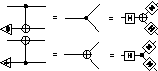
\includegraphics[width=0.5\textwidth]{tensors-from-cn}
\end{center}
These types of identities are common when considering interacting quantum observables \cite{CD, redgreen} as well as quantum circuits \cite{CD, redgreen,BB11}. 
\end{remark}


\begin{example}[\GHZ-class circuits]
We can realize the \GHZ-sate by the following circuit: 
 \begin{center}
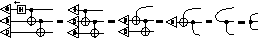
\includegraphics[width=.95\textwidth]{GHZ-state}
\end{center}
The simplification from left to right is a sequence of contractions \cite{BB11}, which recover 
the familiar form of the \COPY-tensor.  On the other hand, one could also realize \GHZ{} by bending a wire as follows. 
 \begin{center}
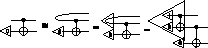
\includegraphics[width=0.80\textwidth]{GHZ-copy}
\end{center}
These circuits scale to create $n$-qubit \GHZ-states in the evident way. 
\end{example}

\begin{example}[Transformations of the controlled Z-gate \cite{CD}]
The following illustrates (graphically) the well known identity that there is a symmetry between the control and target on a controlled Z-gate.  This sequence of rewrites is a law relating \COPY- and \XOR-tensors.  
  \begin{center}
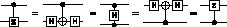
\includegraphics[width=0.75\textwidth]{Zgate}
\end{center}
Such a transformation is common in applications of graphical rewrite systems to measurement based quantum computation \cite{DP10} and appeared in the early work \cite{CD}. 
\end{example}

Now we will recall Lafont's diagrammatic presentation of the bialgebra law, between contractions of \COPY- and \XOR-tensors.  This relationship also appeared in early work on the ZX-calculus in \cite{CD, redgreen}. 

\begin{definition}[\COPY{} and \XOR-tensors form a (scaled) bialgebra \cite{boolean03}]
As mentioned, we often consider {\it equality} as being up to a scalar.  One can think of the bialgebra law as a type of commutation relationship amongst tensor pairs \cite{boolean03}---see early applications to quantum computing in \cite{CD,redgreen} which defined the {\it scaled} bialgebra law.  Turning it side ways we have (ignoring relative scale factors)
\begin{center}
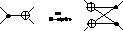
\includegraphics[width=0.4\textwidth]{bialgebra}
\end{center}
\end{definition}


\begin{myexercise}[\COPY{} and \XOR-tensors form a bialgebra \cite{boolean03}]
Verify that \COPY{} and \XOR-tensors form a bialgebra \cite{boolean03}, up to a global scale factor, which should be determined.   
\end{myexercise}


We will now relate this abstract definition to well known quantum circuit identities.  Let us first recall the well known factorization of the \swap{} gate into a triple product of \CNOT-gates.  

\begin{example}[Factorization of the \swap-gate]
As can be shown using the \XOR-algebra (Appendix \ref{sec:XOR}), the \CN-gate together with its horizontally mirrored pair allows one to construct the \swap-gate as follows.  
\begin{center}
 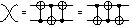
\includegraphics[width=0.40\textwidth]{swap}
\end{center}
A fully graphical proof of this relationship first appeared in the 2008 work \cite{CD} which introduced what is now called the ZX-calculus--see also \cite{redgreen}. 
\end{example}

\begin{theorem}[Relating \swap{} and the scaled bialgebra law] 
In the past, we have provided a diagrammatic proof that the square of the controlled not gate is equal to the identity.  This in turn allows one to relate the \swap-gate (using its factorization above) and the bialgebra law.  
\begin{center}
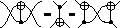
\includegraphics[width=0.36\textwidth]{bialgebra-from-swap}
\end{center}
So the factorization of \swap{} together with \CN$^2=\I$ is enough to have the bialgebra law on tensors.  
\end{theorem}

We will now introduce the gate-copy rewrite rule. Gate-copy allows one to
\textit{pull} controls and targets through each other.  When this happens, they are
copied, along with the attaching wires, leaving the attaching tensor intact.  

\begin{myfullpage}
\begin{theorem}[Gate-copy] 
\label{theorem:gatecopy}
The following graphical rewrites in (a) and (b) hold.    
 \begin{center}
 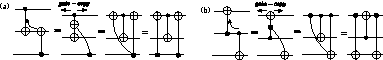
\includegraphics[width=1\textwidth]{gate-copy} 
\end{center}
\begin{proof}
The proof of gate-copy follows from application of the bialgebra and fusion laws, as follows.     
 \begin{center}
 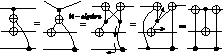
\includegraphics[width=0.65\textwidth]{proof-gate-copy} 
\end{center}
\end{proof}
\end{theorem}
\end{myfullpage}





 \begin{fullpage}
 \begin{example}[Circuit simplification using gate-copy]\label{fig:ZZZsim}
Here we apply gate-copy to simplify the circuit from~\cite{NC} designed to
simulate time evolution under the $\sigma^z\sigma^z\sigma^z$ Hamiltonian.
\end{example}
 \begin{center}
   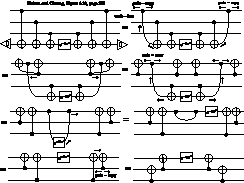
\includegraphics[width=.95\textwidth]{hamexample} %
 \end{center}
Starting from the circuit from Figure 4.19 on page 210 of~\cite{NC}, we
apply a sequence of transformations including the Gate-copy reduction rule introduced in
Theorem~\ref{theorem:gatecopy}.  The network resulting from the simplification appears in the bottom
right. \\ 
\end{fullpage}



\paragraph{Hopf law.}  We recall Lafont's diagrammatic form of the Hopf-law \cite{boolean03}.  

\begin{theorem}[\COPY- and \XOR-tensors satisfy the Hopf-law \cite{boolean03}] 
The following diagrammatic equations, reproduced from \cite{boolean03}, depict the Hopf-law, which is satisfied by \COPY- and \XOR.  
\begin{center}
 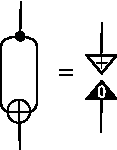
\includegraphics[width=0.12\textwidth]{hopf-law-lafont} 
\end{center}
Exploration of the consequences of this identity in terms of quantum circuit manipulation can be found in the ZX-calculus \cite{redgreen} as well as other works on categorical models of quantum circuits \cite{BB11}. 
\end{theorem}

Using the Hopf law, we can justify a well known gate identity.  This identity was generalized to arbitrary finite dimensions in \cite{BB11}.  
\begin{center}
 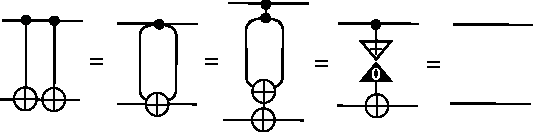
\includegraphics[width=0.5\textwidth]{cn-squared} 
\end{center}

We have considered the key properties and defining equations of the \XOR- and \COPY-tensors.  We will use these results as 
building blocks for the sections that follow on from here. 

\section{Stabilizer Tensor Theory} \label{sec:stabtt}
Let us recall the notation of a stabilizer.  \marginnote{{\it ``We may always depend on it that algebra, which cannot be translated into good English and sound common sense, is bad algebra.'' --- William Kingdon Clifford}}

\begin{definition}[General stabilizer]
A unitary map $U$ stabilizes a quantum state $\psi$ iff 
\begin{equation}
U\psi = (+1)\psi. 
\end{equation} 
Stabilizers of $\psi$ from a group represented trivially by $\psi$.  
\end{definition}

We are concerned here with a subclass of the above definition.  We are concerned with what are commonly known as ``stabilizer states''.  

\begin{definition}[Stabilizer state]
 An $n$-qubit stabilizer state $\psi$ is defined by $n$ commuting and different operators $\1 S$ formed from the Pauli algebra with presentation
 \begin{equation}
     \{\I, X, Y, Z, \pm i, \cdot , \otimes\}. 
 \end{equation}
These $n$ operators generate the stabilizer group of order $2^n$ for $\psi$.   Clearly we have that $s\psi = \psi, \forall s\in \1 S$.    
\end{definition}

\begin{example}[Single qubit stabilizer states]
Here are the single qubit states stabilized by the Pauli-group
\begin{itemize}\addtolength{\itemsep}{-0.25\baselineskip}
 \item[(i)] \textbf{Pauli-X}: $\sigma^x$ stabilizes $\ket{+}=\ket{0}+\ket{1}$
and $-\sigma^x$ stabilizes $\ket{-}=\ket{0}-\ket{1}$
 \item[(ii)] \textbf{Pauli-Y}: $\sigma^y$ stabilizes
$\ket{y_+}=\ket{0}+i\ket{1}$ and $-\sigma^y$ stabilizes
$\ket{y_-}=\ket{0}-i\ket{1}$
 \item[(iii)] \textbf{Pauli-Z}: $\sigma^z$ stabilizes $\ket{0}$ and $-\sigma^z$
stabilizes $\ket{1}$
\end{itemize}
\end{example}

The following is simply a reminder of the essential properties of the Pauli operators.  These are useful for general knowledge and for working through the details of later calculations, but could be skimmed on a first read.  


\begin{definition}
 Recall from angular momentum theory, the familiar Pauli Matrices.  We let $\sigma_1\equiv\sigma_x$, $\sigma_2\equiv\sigma^y$ and $\sigma_3\equiv\sigma^z$ which satisfy 
 \begin{itemize}
  \item[(i)] $[\sigma_i,\sigma_j] = 2i\epsilon^{ijk}\sigma_k$
  \item[(ii)] complex conjugation is generated by $\sigma_j$ $\forall w\in \{i,j,k\}$ as $\sigma_j\sigma_{w}^*\sigma_j=-\sigma_w$ for $w\neq j$
  \item[(iii)] $\text{Tr}(\sigma_i\sigma_j)=2\delta_{ij}$
 \end{itemize}
 Note that it is common to change subscripts to superscripts $\sigma_x\equiv\sigma^x$ to distinguish powers of operators $\sigma_x^2$ from operators acting on specific indices $\sigma^x_3$ --- that is, $\sigma_x$ acting on the third qubit and not $\sigma_x$ cubed.  This should be evident from context.
\end{definition}

These familiar operators from quantum mechanics form what is called a Geometric Algebra (a.k.a. Clifford Algebra). Consider $\{\sigma^l_i\}$ as a basis for a real left and right distributive vector space, such that
\begin{equation}\label{eqn:geometric1}
\sigma_x^2=\sigma_y^2=\sigma_z^2=\I=-i\sigma_x\sigma_y\sigma_z.
\end{equation}
Then consider the product
\begin{equation}\label{eqn:geoprod}
 \sigma_i\sigma_j = \delta_{ij}\I + i\epsilon^{ijk}\sigma_k~~~\text{(geometric product of vectors)}.
\end{equation}
It is clear that for $i\neq j$
\be \label{eqn:vanish}
\{\sigma_i^l,\sigma_j^l\}=0
\ee
meaning that the vectors anti-commute viz.,
\be \label{eqn:anti}
\sigma_i^l\sigma_j^l=-\sigma_j^l\sigma_i^l.
\ee
We also note that 
\be \label{eqn:eyepauli}
\{\sigma^i,\sigma^j\}=2\delta_{ij}\I.
\ee

\begin{myexercise}
 Verify Equations~\eqref{eqn:geoprod}, \eqref{eqn:vanish}, \eqref{eqn:anti} and \eqref{eqn:eyepauli}. 
\end{myexercise}


Single qubit density operators can be expanded in terms of a dot product of a polarisation vector $\underline{P} :=(p_1,p_2,p_3)$, $\forall i, p_i \in \7 R$, and a sigma vector $\underline{\sigma}:= (\sigma_1, \sigma_2,\sigma_3)$ as
\begin{equation}
\rho = \frac{1}{2}\I + \underline{\sigma}.\underline{P} =\frac{1}{2}\I +  p_i\sigma^i = p_1\sigma^1 + p_2\sigma^2 + p_3\sigma^3. 
\end{equation}  

Clearly the vectors $\underline{P}$ are in the vector space $\7 R^3$.  We can elevate this vector space to a Hilbert space by defining an inner product between vectors --- that is a map $(-,-)$ taking two elements from the vector space (in this case Hamiltonians on $\7C^2$) and producing a scalar in the underlining field $\7C$.
\begin{equation*}
 (-,-):(\7C^2\rightarrow\7C^2)\times(\7C^2\rightarrow\7C^2)\rightarrow \7C
\end{equation*}
\be 
(\underline{\sigma}.\underline{A}, \underline{\sigma}.\underline{B})\mapsto Tr[(\underline{\sigma}.\underline{A}).(\underline{\sigma}.\underline{B})] = \underline{A}.\underline{B}
\ee 


\begin{myexercise}[Product of vectors] 
 Verify that straight forward calculation also yields
\be
(\underline{\sigma}.\underline{A},\underline{\sigma}.\underline{B})=A_iB_i + i\epsilon_{ijk}\sigma^k = \underline{A}.\underline{B} + i\underline{\sigma}(\underline{A}\wedge \underline{B}).
\ee
\end{myexercise}



\begin{myexercise}[Eigenvalues] 
 Verify, by using the fact that for $\underline{A}=\underline{B}$ the cross product vanishes or otherwise, that the eigenvalues of $(\underline{A}.\underline{\sigma})$ are $\pm|\underline{A}|$, where both roots necessarily appear as $\underline{A}.\underline{\sigma}$ is traceless. 
\end{myexercise}


We can relate symmetry in density operators and symmetry in states as follows.  

\begin{comment}
\begin{remark}[Symmetric density operators vs symmetric states]
A symmetric single qubit density operator necessarily has $bY=0$ and so gives rise by bending wires to a symmetric two qubit state with real valued coefficients parametrized by two real degrees of freedom, $\psi_\rho(a, 0, c)$.  Diagrammaticality, a symmetric two-party state (a) is invariant under exchange of its legs whereas a symmetric density operator is invariant under exchange of its arms and legs (e.g. transpose as in (b)).  
\begin{center}
 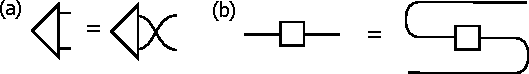
\includegraphics[width=10\xxxscale]{2-party-symmetric-states1}
\end{center}
\end{remark}
\end{comment}

Before continuing on to define the Clifford group of quantum circuits, we will consider an example of a stabilizer state.  

\begin{example}[The Bell state is a stabilizer state]
 The bell state 
 \be 
 \Phi^+ = \sum a \oplus \neg b \ket{a, b} = \ket{00}+\ket{11}
 \ee 
 is a stabilizer state with stabilizer group 
 \be 
 \1S= \{\I, XX, -YY, ZZ\}
 \ee 
Note that this matches the following claims in the definition (i) the stabilizer group is of order $2^n$, here $n=2$, with generators given by e.g. $XX$, $ZZ$, etc. and (ii) the group is abelian.  
\end{example}


\begin{myexercise}
 Verify that $XX$, $-YY$ and $ZZ$ are in fact stabilizers of the Bell state $\Phi^+$ graphically.  
 Using the rules of the Pauli algebra, verify that these operators commute.  
\end{myexercise}



\begin{myexercise}
 Find the stabilizers for the following states.  
 \be 
 \Phi^- = \ket{00}-\ket{11}
 \ee 
 \be 
 \Psi^- = \ket{01}-\ket{10}
 \ee 
 Hint.  One method would be to use the Pauli algebra and the stabilizes for $\Psi^+$.  First cancel the local operator separating the given states from 
 $\Psi^-$, apply the known stabilizer and then reapply the operator to return to the starting state.  Other methods exist. 
\end{myexercise}


\section{The Clifford Group}

\marginnote{{\it 
The following are equivalent. 
\begin{itemize}
    \item[1.] The ZX-calculus \cite{Coecke2017}.
    \item[2.] Clifford gates plus cups and caps. 
    \item[3.] Ability to bend wires and compose stabilizer states.
\end{itemize}
}}

There is another useful way of generating stabilizer states.  We will consider a quantum circuit acting on the state $\ket{0}^{\otimes n}$.  The circuit is comprised solely of Clifford gates.

\begin{definition}[Clifford gates]
The collection of Clifford gates is as follows. (a) \CNOT{}; (b) the Hadamard gate $H = \frac{1}{\sqrt{2}}(X+Z)$; (c) The phase gate $P = \ket{0}\bra{0} + i \ket{1}\bra{1}$, and (d) the Pauli gates generated by the Pauli algebra on a single qubits, with 16 elements (the group generated by $\{X, Y, Z\}$).    
 \begin{center}
 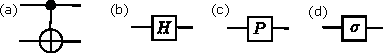
\includegraphics[width=0.65\textwidth]{clifford-gates} 
\end{center}
\end{definition}

\begin{remark}[Single qubit Clifford group]
The standard properties of single qubit gates follow. 
\begin{itemize}
 \item[(i)] $HXH=Z$; and $HZH = X$
 \item[(ii)] $PXP^\dagger = Y$; and $PYP^\dagger = Z = P^2$
\end{itemize}
These gates above generate the single qubit Clifford group.   
\end{remark}

With the definitions of the Clifford group in place, one can state the alternative definition of stabilizer states.  

\begin{definition}[Stabilizer states]
If $\psi$ can be produced from the all-$\ket{0}$ state by Clifford gates, then $\psi$ is stabilized by $2^n$ tensor products of Pauli matrices or their sign opposites (where $n$ is the number of qubits).  This means that the stabilizer group is generated by $\log(2^n)=n$ such tensor products.  The state $\psi$ is then the \textit{stabilizer state} uniquely determined by these generators.
\end{definition}

\begin{remark}[Properties of Clifford circuits]
We now list elementary properties of Clifford circuits.  
 \begin{itemize}
  \item[(i)] Clifford circuits generate the Clifford group.
  \item[(ii)] Let $P_n$ be the collection of $4^n$ $n$-letter words with $\otimes$ as concatenation generated from the alphabet
  \begin{equation}
      \{\pm\I, \pm X,\pm Y,\pm Z, \pm i\I, \pm iX,\pm iY,\pm iZ\}. 
  \end{equation}
All operators $g$ in the Clifford group acts as an involution when $P_n$ is conjugated by $g$, that is $g P_n g^\dagger = P_n$.    
 \item[(iii)] Note, alternative notation to write $P_1$ could be 
 \be 
 P_1 = \{\pm 1, \pm i\}\{\I, X, Y, Z\}. 
 \ee
 \item[(iv)] Defining properties of the Pauli matrices:
 \begin{equation}
     X^2=Y^2=Z^2=\I = -iXYZ.
 \end{equation}
  \end{itemize}
\end{remark} 


\begin{myexercise}
 Show that conjugation by $H$ lifts to an involution on $P_1$ by considering (iv) with $H= \frac{1}{\sqrt{2}}(Z+X)$.
\end{myexercise}


\section{Stabiliser Tensor Theory}

Let us cast the stabilizer theory into a theory of tensors, in the Penrose graphical calculus.  We will first define the notation of an abstract stabilizer for a tensor.  

\begin{definition}[Abstract stabilizer]
 Let $\Gamma$ be a valence-($n$,$m$) tensor.  A stabilizer for $\Gamma$ is given by $m+n$ local invertible operators, satisfying 
  \begin{center}
 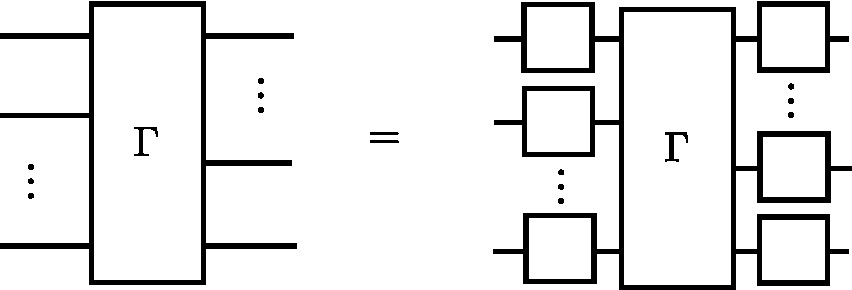
\includegraphics[width=0.5\textwidth]{tensor-stabs} 
\end{center}
\end{definition}

We then turn to a definition of tensors, which as we will soon show, generate the Clifford circuits as a subclass.  

\begin{theorem}[Stabilizer tensors]
Contraction of tensors taken from the following are sufficient to generate the stabilizer group.  
\begin{center}
 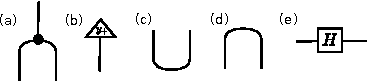
\includegraphics[width=0.5\textwidth]{stab-tensor-generators} 
\end{center}
Where (a) is the \COPY-tensor, (b) is the y-plus-state $\ket{y_+}\bydef\ket{0}+i\ket{1}$, the cup (c) and cap (d) are to bend wires and hence reshape maps and take transposes, (e) is the Hadamard gate.  
\begin{proof}[Stabilizer tensors]
 Let us first consider generating the states $\ket{+}$, $\ket{-}$, $\ket{y_-}$. These are found from the following tensor contractions.
\begin{center}
 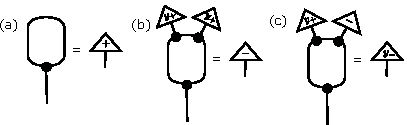
\includegraphics[width=0.5\textwidth]{state-generators1} 
\end{center}
From these states, the following contractions generate our elementary gates.
\begin{center}
 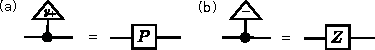
\includegraphics[width=0.5\textwidth]{gate-generators} 
\end{center}
We then note that 
\be 
HZH = X
\ee 
\be 
P^\dagger = P^2P 
\ee 
and that 
\be 
PXP^\dagger = PXP^3 = Y
\ee 
We recover the \COPY-tensor by contracting with Hadamard gates and \CNOT{} is found from reshapes of the following contraction
\begin{center}
 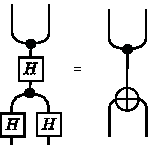
\includegraphics[width=0.16\textwidth]{cnot-contraction1} 
\end{center}
We then recover the generators of the Clifford group.   
\end{proof}
\end{theorem}



Now we will consider stabilizers of the \COPY-tensor.  

\begin{example}[Stabilizers of \COPY] The \COPY-tensor has stabilizer
generators $\sigma^x_1\otimes\sigma^x_2\otimes\sigma^x_3$ and
$\sigma^z_i\otimes\sigma^z_j$ which uniquely determine
$\psi_{GHZ}=\ket{000}+\ket{111}$ and result in the following stabilizer group of order $2^3=8$. 
\be
\{\sigma^x\sigma^x\sigma^x,-\sigma^x\sigma^y\sigma^y,
-\sigma^y\sigma^x\sigma^y,-\sigma^y\sigma^y\sigma^x,
\I\otimes \sigma^z\otimes\sigma^z,\sigma^z\otimes\I\otimes \sigma^z,
\sigma^z\otimes\sigma^z\otimes\I, \I\}
\ee 
Diagrammatically these relations are given in Figure~\ref{fig:stabGHZ}.   

\end{example}


\begin{figure}[h]
\centering
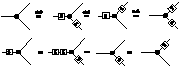
\includegraphics[width=0.7\textwidth]{Zstabs}\\
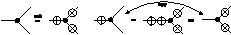
\includegraphics[width=0.750\textwidth]{Xstabs}\\
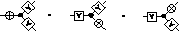
\includegraphics[width=0.60\textwidth]{XstabsYY1}
\caption{(Top) Diagrammatic depiction of the stabilizer equation
$\sigma^z_i\sigma^z_j(\ket{000}+\ket{111})=\ket{000}+\ket{111}$. (Bottom)
Uses the stabilizer identity together with $\sigma_z^2=\I$ to show that
the $\sigma^z$ commutes with the \COPY-tensor. (Middle) Diagrammatic depiction of the stabilizer
equation
$\sigma^x_1\otimes\sigma^x_2\otimes\sigma^x_3(\ket{000}+\ket{111})=\ket{000
}+\ket{111}$.  (Bottom) Diagrammatic depiction (up to a sign) of the
stabilizer equation
$-\sigma^x_i\otimes\sigma^y_j\otimes\sigma^y_k(\ket{000}+\ket{111})=\ket{
000}+\ket{111}$.} 
\label{fig:stabGHZ}
\end{figure}




\begin{myexercise}[Gottesman-Knill Theorem] 
A graphical rewrite proof (by bounding the number of rewrites) of the
Gottesman-Knill theorem follows by considering the action of the \COPY- and \XOR-tensors on $\sigma^z$ and $\sigma^x$.  Derive the gate identities in paper \cite{GN98} and 
prove the main theorem using the methods from this lecture.  
\end{myexercise}



\begin{myexercise}[Stabilizers for $\delta_{ijkl}$]
Write down the $2^4$ stabilizers of the state 
\be 
 \sum_{ijkl\in\{0,1\}^4} \delta^{ijkl}\ket{ijkl}
\ee 
Now consider stabilizers in (a).  We can expand this arriving at (b).  What are the conditions on $C$ and $D$ such that $A$, $B$, $E$, $F$ are stabilizers?  Compare this with the 
stabilizers given for \COPY, prior to contraction.  
\begin{center}
 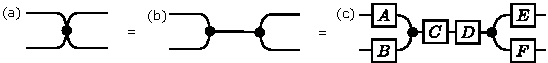
\includegraphics[width=0.65\textwidth]{4-party-stabs} 
\end{center}
\end{myexercise}

We can now consider how stabilizers of a tensor transform, when the tensor undergoes a local change of basis.  

\begin{theorem}[Transformation properties of stabilizers]
Let $\Gamma$ be a tensor with stabilizer $A\otimes B\otimes \cdots \otimes C$.   Then if we rotate $\Gamma$ as 
$\Gamma' = U_G(\Gamma)$, then 
\be
U_G(A\otimes B\otimes \cdots \otimes C) = U_G(A)\otimes U_G(B)\otimes \cdots \otimes U_G(C)
\ee
is a stabilizer for $\Gamma'$.  
\end{theorem}





\section{Boolean Stabilizer States}

Now one can consider the intersection found from the class of Boolean states which are in addition to being Boolean states, also stabilizer states.  We will construct them explicitly for the case of a single qubit, and leave the two qubit case 
as homework.  

\section*{Single qubit Boolean Stabilizer States}

There is one stabilizer state for each single qubit boolean state.  This correspondence is a special case 
of the dim $=2$ state space and does not hold in any higher dim.  \marginnote{{\it ``To know all about anything is to know how to deal with it under all circumstances.'' --- 
William Kingdon Clifford} }


\subsection*{Single bit functions} 
Consider 
\be 
f:\7 B^2 \rightarrow \7 B 
\ee 
then a general function $f$ is expanded as a sum-of-products (LHS) and as a pseudo Boolean form (RHS)  
\be 
c_0 \overline{x}\vee c_1 x = c_0 + (c_1 - c_0)x 
\ee 
for $c_0, c_1, x \in \7 B$.  There are exactly $2^{2^n}$ boolean functions.  Evaluated at $n=1$ gives four possible single qubit Boolean states.  One of these however, corresponds to 
$\psi =0$ and so is trivial.  The others are $\ket{0}$, $\ket{1}$ and $\ket{0}+\ket{1}$.  

\subsection*{Single qubit stabilizer operators} 

We will consider $\pm Z$ and $X$.  These are the only possible stabilizer operators that stabilize single qubit boolean states.  
\be 
X(c_0\ket{0} + c_1\ket{1}) = c_1 \ket{1} + c_0 \ket{0} 
\ee 
and hence, $X\psi = +1 \psi$ iff $c_1 = c_0$.  Over $\7B$ this has non-trivial solutions (that is, $\|\psi\| > 0$) for 
$c_0=c_1=1$ and hence, we recover the only boolean state stabilized by $X$ as $\ket{0}+\ket{1}$.  We will then consider 
\be 
\pm Z \psi = \pm c_0 \ket{0} \mp c_1 \ket{1} 
\ee 
and $\pm Z \psi = +1 \psi$ iff $\pm c_0 = \mp c_1$.  It follows that 
\be 
+ Z \Rightarrow c_0 = 1, c_1 = 0 
\ee 
\be 
-Z \Rightarrow c_0 = 0, c_1 = 1
\ee 

\subsection*{Correspondence between stabilizer states and boolean states} 

In this section we consider the correspondence between single qubit stabilizer states and single 
qubit boolean states.  Let us introduce two boolean variables, $b_0$ and $b_1$.  We then write 
\be 
(-1)^{b_1}(1-b_0)Z + b_0 X
\ee 
We find that $b_0$ $\Rightarrow$ $c_0=c_1=1$.  The case that $b_0=0$ implies that $b_1$ decides $c_0, c_1$ as 
\be 
b_1=1 \Rightarrow c_1=1, c_0=0
\ee 
\be
b_1=0 \Rightarrow c_1=0, c_0=1
\ee 
We will then parameterize the single qubit boolean state in terms of $b_0$ and $b_1$ as 
\be 
\psi_{\7 B} = (b_0 \vee\overline b_0 \wedge b_1)\ket{0} + (b_0\vee \overline b_0 \wedge \overline b_1)\ket{1} = (b_0 + b_1-b_0b_1)\ket{0} + (1+b_0 - b_1 + b_0b_1)\ket{1}
\ee 
and hence the choice $c_0 = b_0 + b_1-b_0b_1$ and $c_1 = 1+b_0 - b_1 + b_0b_1$ provides the correspondence.  

\begin{remark}
 In or around circa.~2010, I discussed development of classification scheme for Boolean stabilizer states with Oscar Dahlsten.  I believed Oscar solved that problem, specifying exactly the class of Boolean stabilizer states. 
\end{remark}



\begin{myexercise}[Two qubit Boolean stabilizer states]
 For two qubits, there are $2^{2^2}-1 = 15$ boolean states.  Let $q$ and $r$ take boolean values.  Then we arrive at the following truth table.  

\begin{center}
\begin{tabular}{l||l|l||l|l|l|l|l|l|l|l|l|l|l|l|l|l}
$q$ $r$ & $f_0$  & $f_1$  &   &   &   &   &   &   &   &   &   &   &   &   &   & $f_\wedge$ \\\hline 
$0$ $0$ & 0 & 1 & 1 & 1 & 1 & 0 & 1 & 1 & 0 & 0 & 1 & 0 & 1 & 0 & 0 & 0 \\
$0$ $1$ & 0 & 1 & 1 & 1 & 0 & 1 & 1 & 0 & 1 & 0 & 0 & 1 & 0 & 1 & 0 & 0 \\
$1$ $0$ & 0 & 1 & 1 & 0 & 1 & 1 & 0 & 1 & 1 & 1 & 0 & 0 & 0 & 0 & 1 & 0 \\
$1$ $1$ & 0 & 1 & 0 & 1 & 1 & 1 & 0 & 0 & 0 & 1 & 1 & 1 & 0 & 0 & 0 & 1
\end{tabular}
\end{center}


\begin{itemize}
 \item[(i)] Label \OR, \NOR, \NAND, \XOR{} in the table above.  
 \item[(ii)] Using the definition of $K_1$, determine which states in this table are separable, and classify them based on the resulting values of $K_1$. 
 \item[(iii)] Which states in the table are not stabilizer states?  
\end{itemize}
\end{myexercise}

\begin{myexercise}[Invariants of symmetric Boolean states]
~
\begin{itemize}
 \item[(i)] Write the general form of a symmetric three qubit boolean state.  How many possible symmetric boolean states are there? 
 \item[(ii)] Consider the discriminant of the cubic.
\be 
\Delta = a_0^2 a_3^2 - 6 a_0 a_1 a_2 a_3 + 4 a_0 a_2^3 - 3a_1^2 a_2^2 + 4 a_1^3 a_3
\ee 
and find maximum and minimum values when $\forall i, a_i\in \{0,1\}$.  
\end{itemize}
\end{myexercise}


\section{Problems} 

\begin{theorem}[Sufficient expression stabilizer states]
Let 
\be 
f, g, k:\7B^n\rightarrow \7B
\ee 
then the quantum state 
\be 
\psi_{\7B} = \sum (-1)^{f(\1 x)}(i)^{g(\1 x)}k(\1 x)\ket{\1 x}
\ee 
is sufficient to express any stabilizer state.  
\begin{proof}[Normal forms on stabilizer states]
 Each stabilizer state is an equally weighted superposition with coefficients $\pm1, \pm i, 0$.  The functions $f, g, k$ determine these for each basis vector 
 $\ket{\1 x}$.  
\end{proof}
\end{theorem}


\begin{remark}[Normal forms]
 Using a PPRM from lecture II, we can expand $f, g, k$ to a normal form.  The functions then become uniquely determined by a coefficient vector.  
\end{remark}



\begin{myexercise}[Stabilizer states as pseudo Boolean forms]
 Find $f$, $g$, and $k$ to express the following states (note, the second is not a stabilizer state). 
 \begin{itemize}
  \item[(i)] $\psi_1 = \ket{000} + i \ket{111}$
  \item[(ii)] $\psi_2 = \ket{001} + i \ket{010} - i\ket{100}$  
 \end{itemize}
\end{myexercise}

\begin{myexercise}[Stabilizer generators]
\marginnote{{\it ``An expert is someone who knows some of the worst mistakes that can be made in their subject and how to avoid them.''}--- Werner Heisenberg}
 Consider $U$ as an arbitrary Clifford circuit.  Then, 
 \be 
 \psi = U\ket{0}^{\otimes n}
 \ee 
 is an arbitrary stabilizer state.  Show that evolution of $Z_i$ under $U$ in the Heisenberg picture
 \be 
 UZ_iU^\dagger
 \ee 
 is necessarily a stabilizer for $\psi$.  
\end{myexercise}

\begin{myexercise}[Further Exercises on Pauli Matricies] 
~
\begin{itemize}
 \item[(i)] Let $\underline{P}.\underline{\sigma} := p_0 X + p_1 Y + p_2 Z$ where $|P|=1$. Show that $\exp(-i\frac{\theta}{2}\underline{P}.\underline{\sigma})=\I \cos(\theta/2)-i(\underline{P}.\underline{\sigma})\sin(\theta/2)$ and find the values of $\theta$, $\underline{P}$ to recover the Hadamard gate, up to a phase factor.  

\item[(ii)] Find the time of the evolution of the Hamiltonian $\ket{11}\bra{11}$ to create a {\sf CZ}-gate, then write down a quantum circuit in terms of {\sf H}  and {\sf CZ} to create a {\sf CNOT}-gate.  What are the input states needed to use the {\sf CNOT}-gate to prepare the singlet state $\ket{\Psi^-}=\ket{01}-\ket{10}$?  

\item[(iii)] Show that the \swap{} operator $\frac{1}{2}(\I + \underline{\sigma}_A\cdot\underline{\sigma}_B)$ permutes the values of bits $A$ and $B$ as 
  \begin{equation}
   \text{\swap} \ket{i_A}\ket{i_B} = \ket{i_B}\ket{i_A}
  \end{equation}
  where the notation $ \underline{\sigma}_A\cdot\underline{\sigma}_B$ is typically said to stand for the scalar and tensor product:  
  $ \underline{\sigma}_A\cdot\underline{\sigma}_B = \sum_{i = 1}^3 \sigma_i^A \otimes \sigma_i^B.$ 

\item[(iv)] In the computational basis, express the general form of a two-qubit symmetric eigenstate of the \swap{} operator and count the real degrees of freedom.  Repeat this for anti-symmetric eigenstates (e.g. $\swap\ket{\psi}=-\ket{\psi}$).  
%  \item[(vi)] Express the SWAP operator as a composition of operators of the form
%  \begin{equation}
%  \eta := \sum_i \ket{i}\otimes \ket{i}
% \end{equation}
% \begin{equation}
%  \epsilon := \sum_i \bra{i}\otimes \bra{i}
% \end{equation}
\item[(v)] Using the notation from (iii) above, find a value for $q$ to show that the two-site quantum Heisenberg model $J\underline{\sigma}_1\cdot \underline{\sigma}_2$ can be written as $\frac{J}{2}\left((\underline{\sigma}_1+\underline{\sigma}_2)^2-q\I\right)$ and show that $\ket{\Psi^\pm}=\ket{01}\pm\ket{10}$ are energy eigenstates.  
\end{itemize}
\end{myexercise}


